\subsection{Failures in PIR Sensors -- A Taxonomy} 
\label{subsec:taxonomy} 

Fundamentally, failures in a PIR sensor could occur either on the lens, the pyroelectric element or the electronics. We \textit{analyze and categorize practical, common and most frequent} failures as gathered in discussions with IoT engineers and technicians who install and maintain PIR sensor deployments. 
We developed a new taxonomy for such failures, as summarized in {\bfseries Table~\ref{tab:pir_faults}} and visualized in {\bfseries Fig.~\ref{fig:pir_sensor_failure_photographs}}.%
%
\subsubsection{\textbf{Failures in the lens subsystem}} The lens is geometrically constructed to precisely focus the thermal rays onto the pyroelectric element. As a result, failures affecting the optical integrity of the lens can result in loss of precision for focusing the thermal rays. We observe three types of failures here, termed Class I--III failures.
%

\noindent \underline{Lens dislocation (Class I):} %
As the lens is stuck on the sensor board with an adhesive or machined to fit over the pyroelectric element, it could get dislodged from its place or completely fall off the sensor board due to factors such as thermal expansion or physical impact.

\begin{figure}%
	\centering
	\small
	\begin{subfigure}[t]{0.24\textwidth}
		\centering
		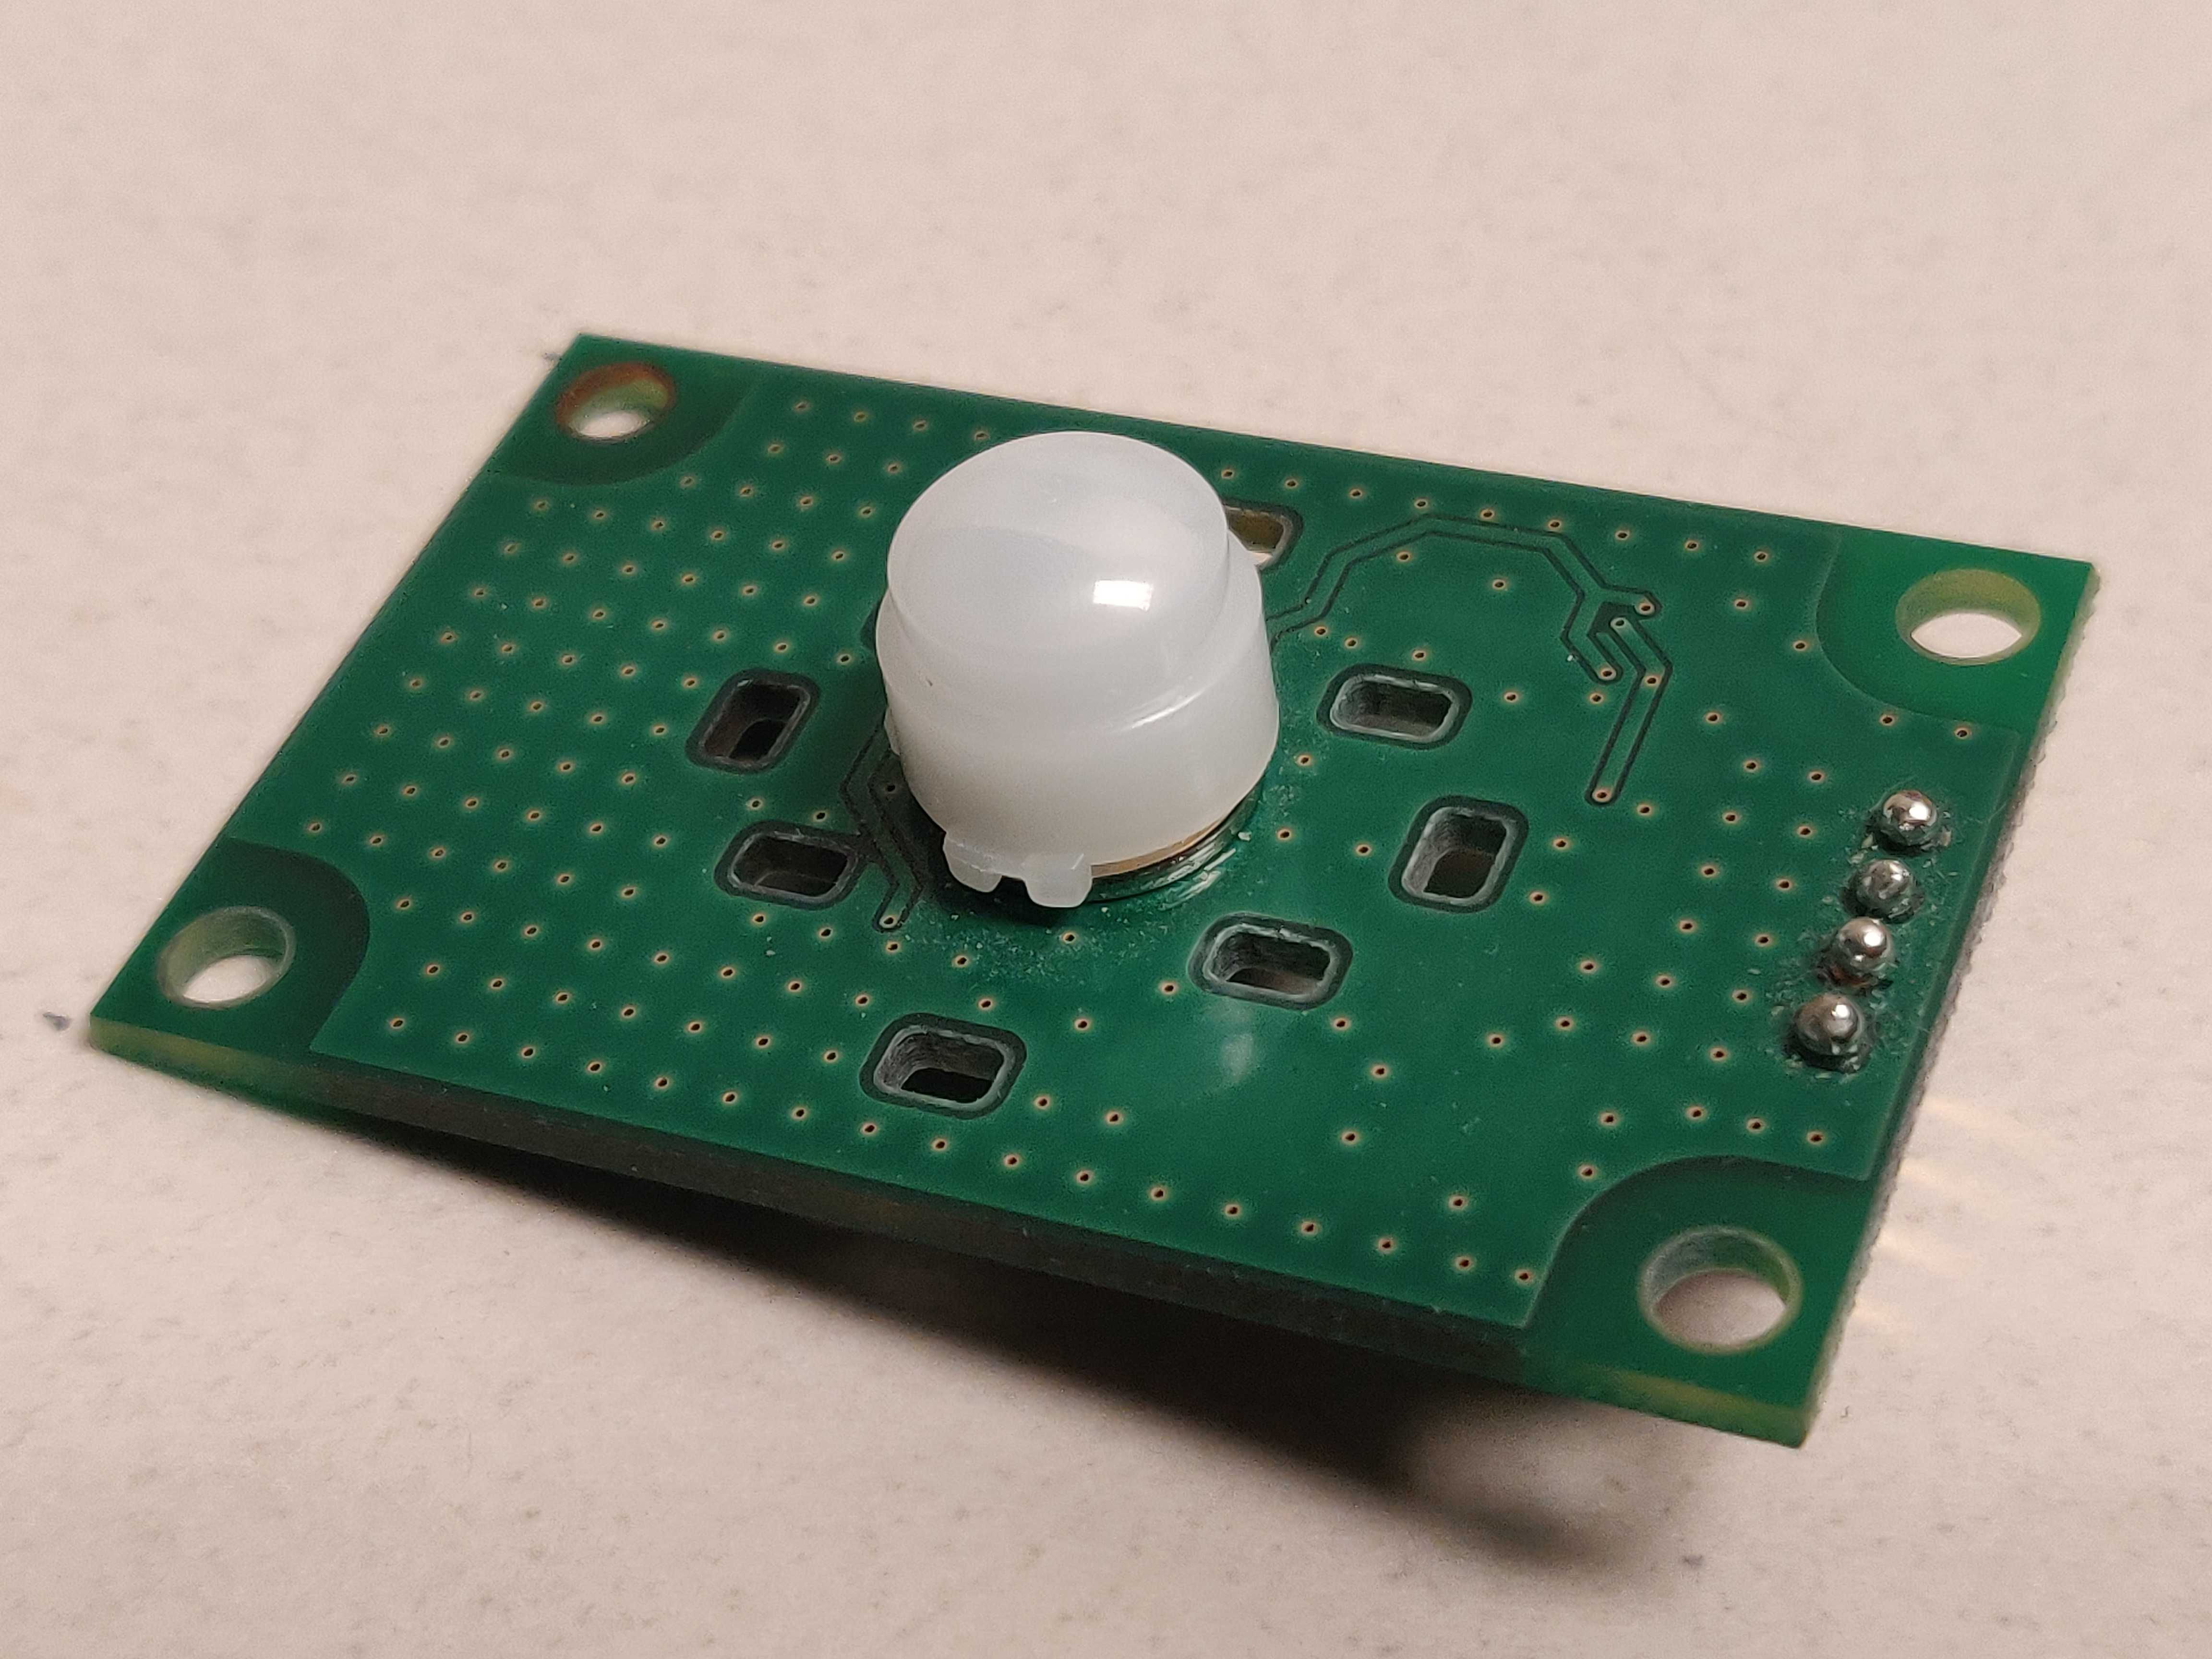
\includegraphics[width=\textwidth]{figures/platform/failure_photographs/WorkingSensor-proper.jpg}
		\caption{\footnotesize Working Sensor}
		\label{fig:working}
	\end{subfigure}
	\hspace{0.10ex}%
	\begin{subfigure}[t]{0.24\textwidth}
		\centering
		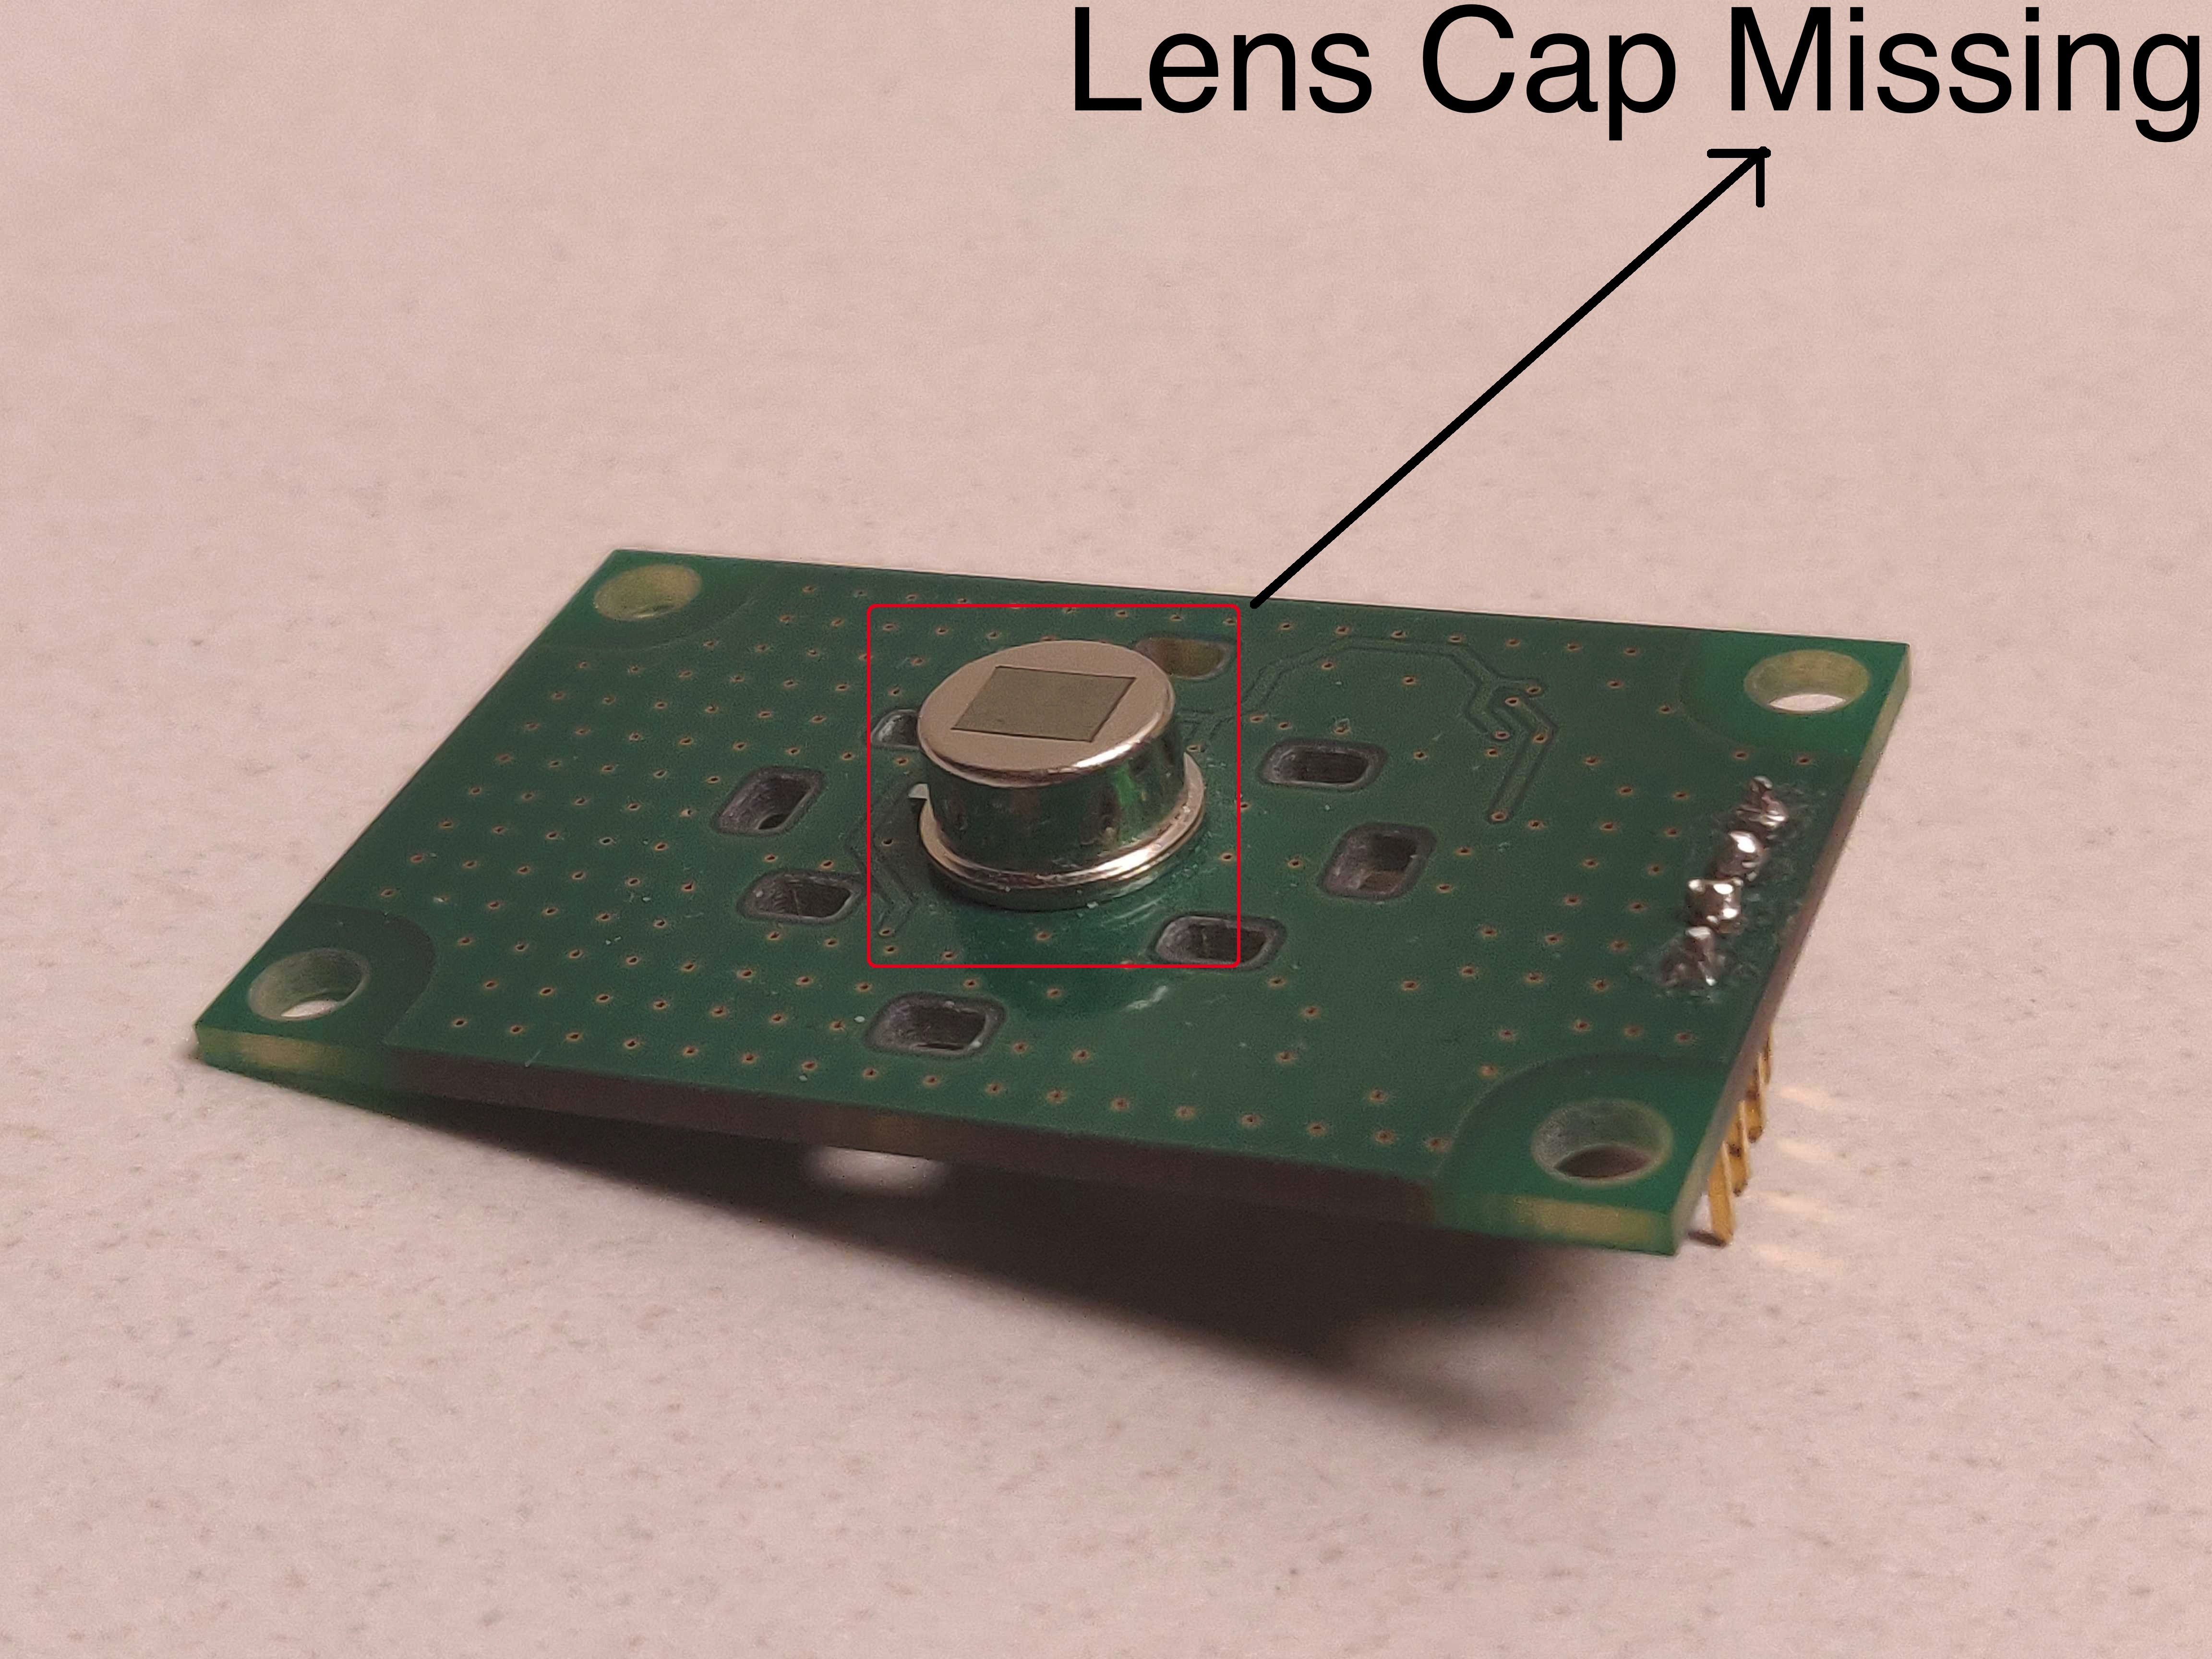
\includegraphics[width=\textwidth]{figures/platform/failure_photographs/ClassI-LensCapRemoved-annotated-jpg.jpg}
		\caption{Lens Cap Fallen Off}
		\label{fig:failure_photo1}
	\end{subfigure}
	\hspace{0.10ex}
	\begin{subfigure}[t]{0.24\textwidth}
		\centering
		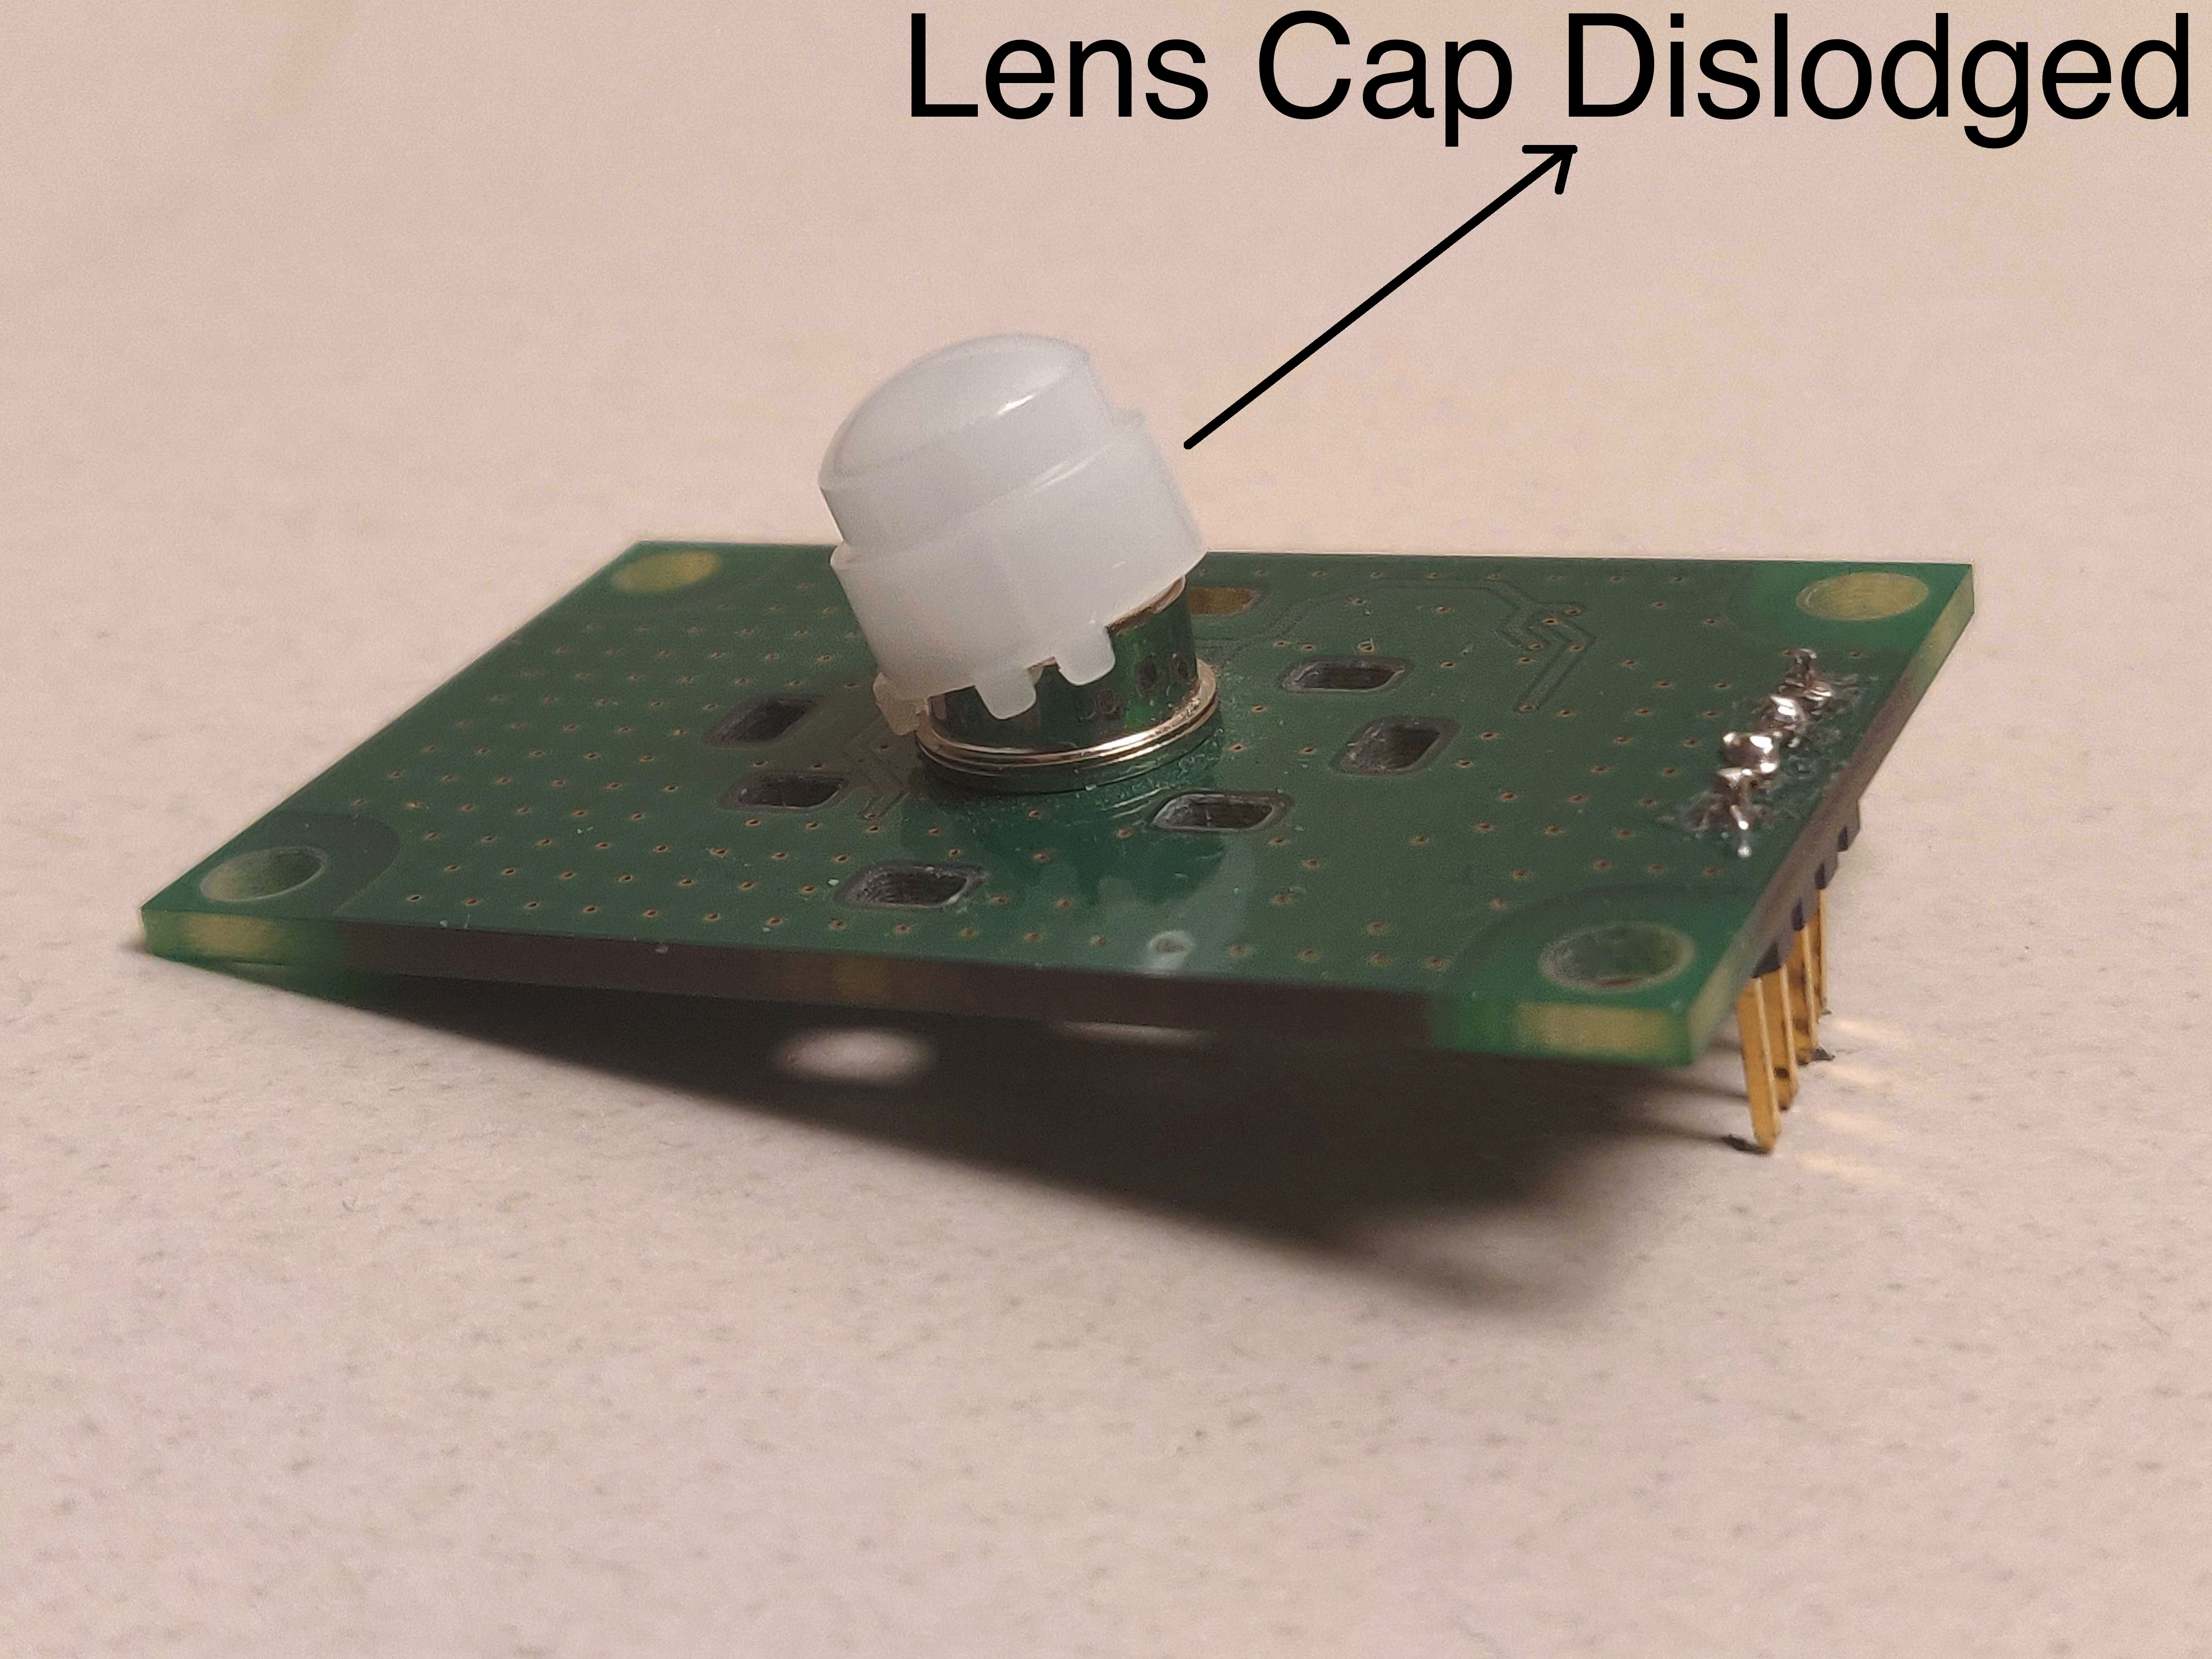
\includegraphics[width=\textwidth]{figures/platform/failure_photographs/ClassI-LensCapDislogdged-annotated-jpg.jpg}
		\caption{\footnotesize Lens Cap Dislocated}
		\label{fig:failure_photo2}
	\end{subfigure}	
	\hspace{0.10ex}
	\begin{subfigure}[t]{0.24\textwidth}
		\centering
		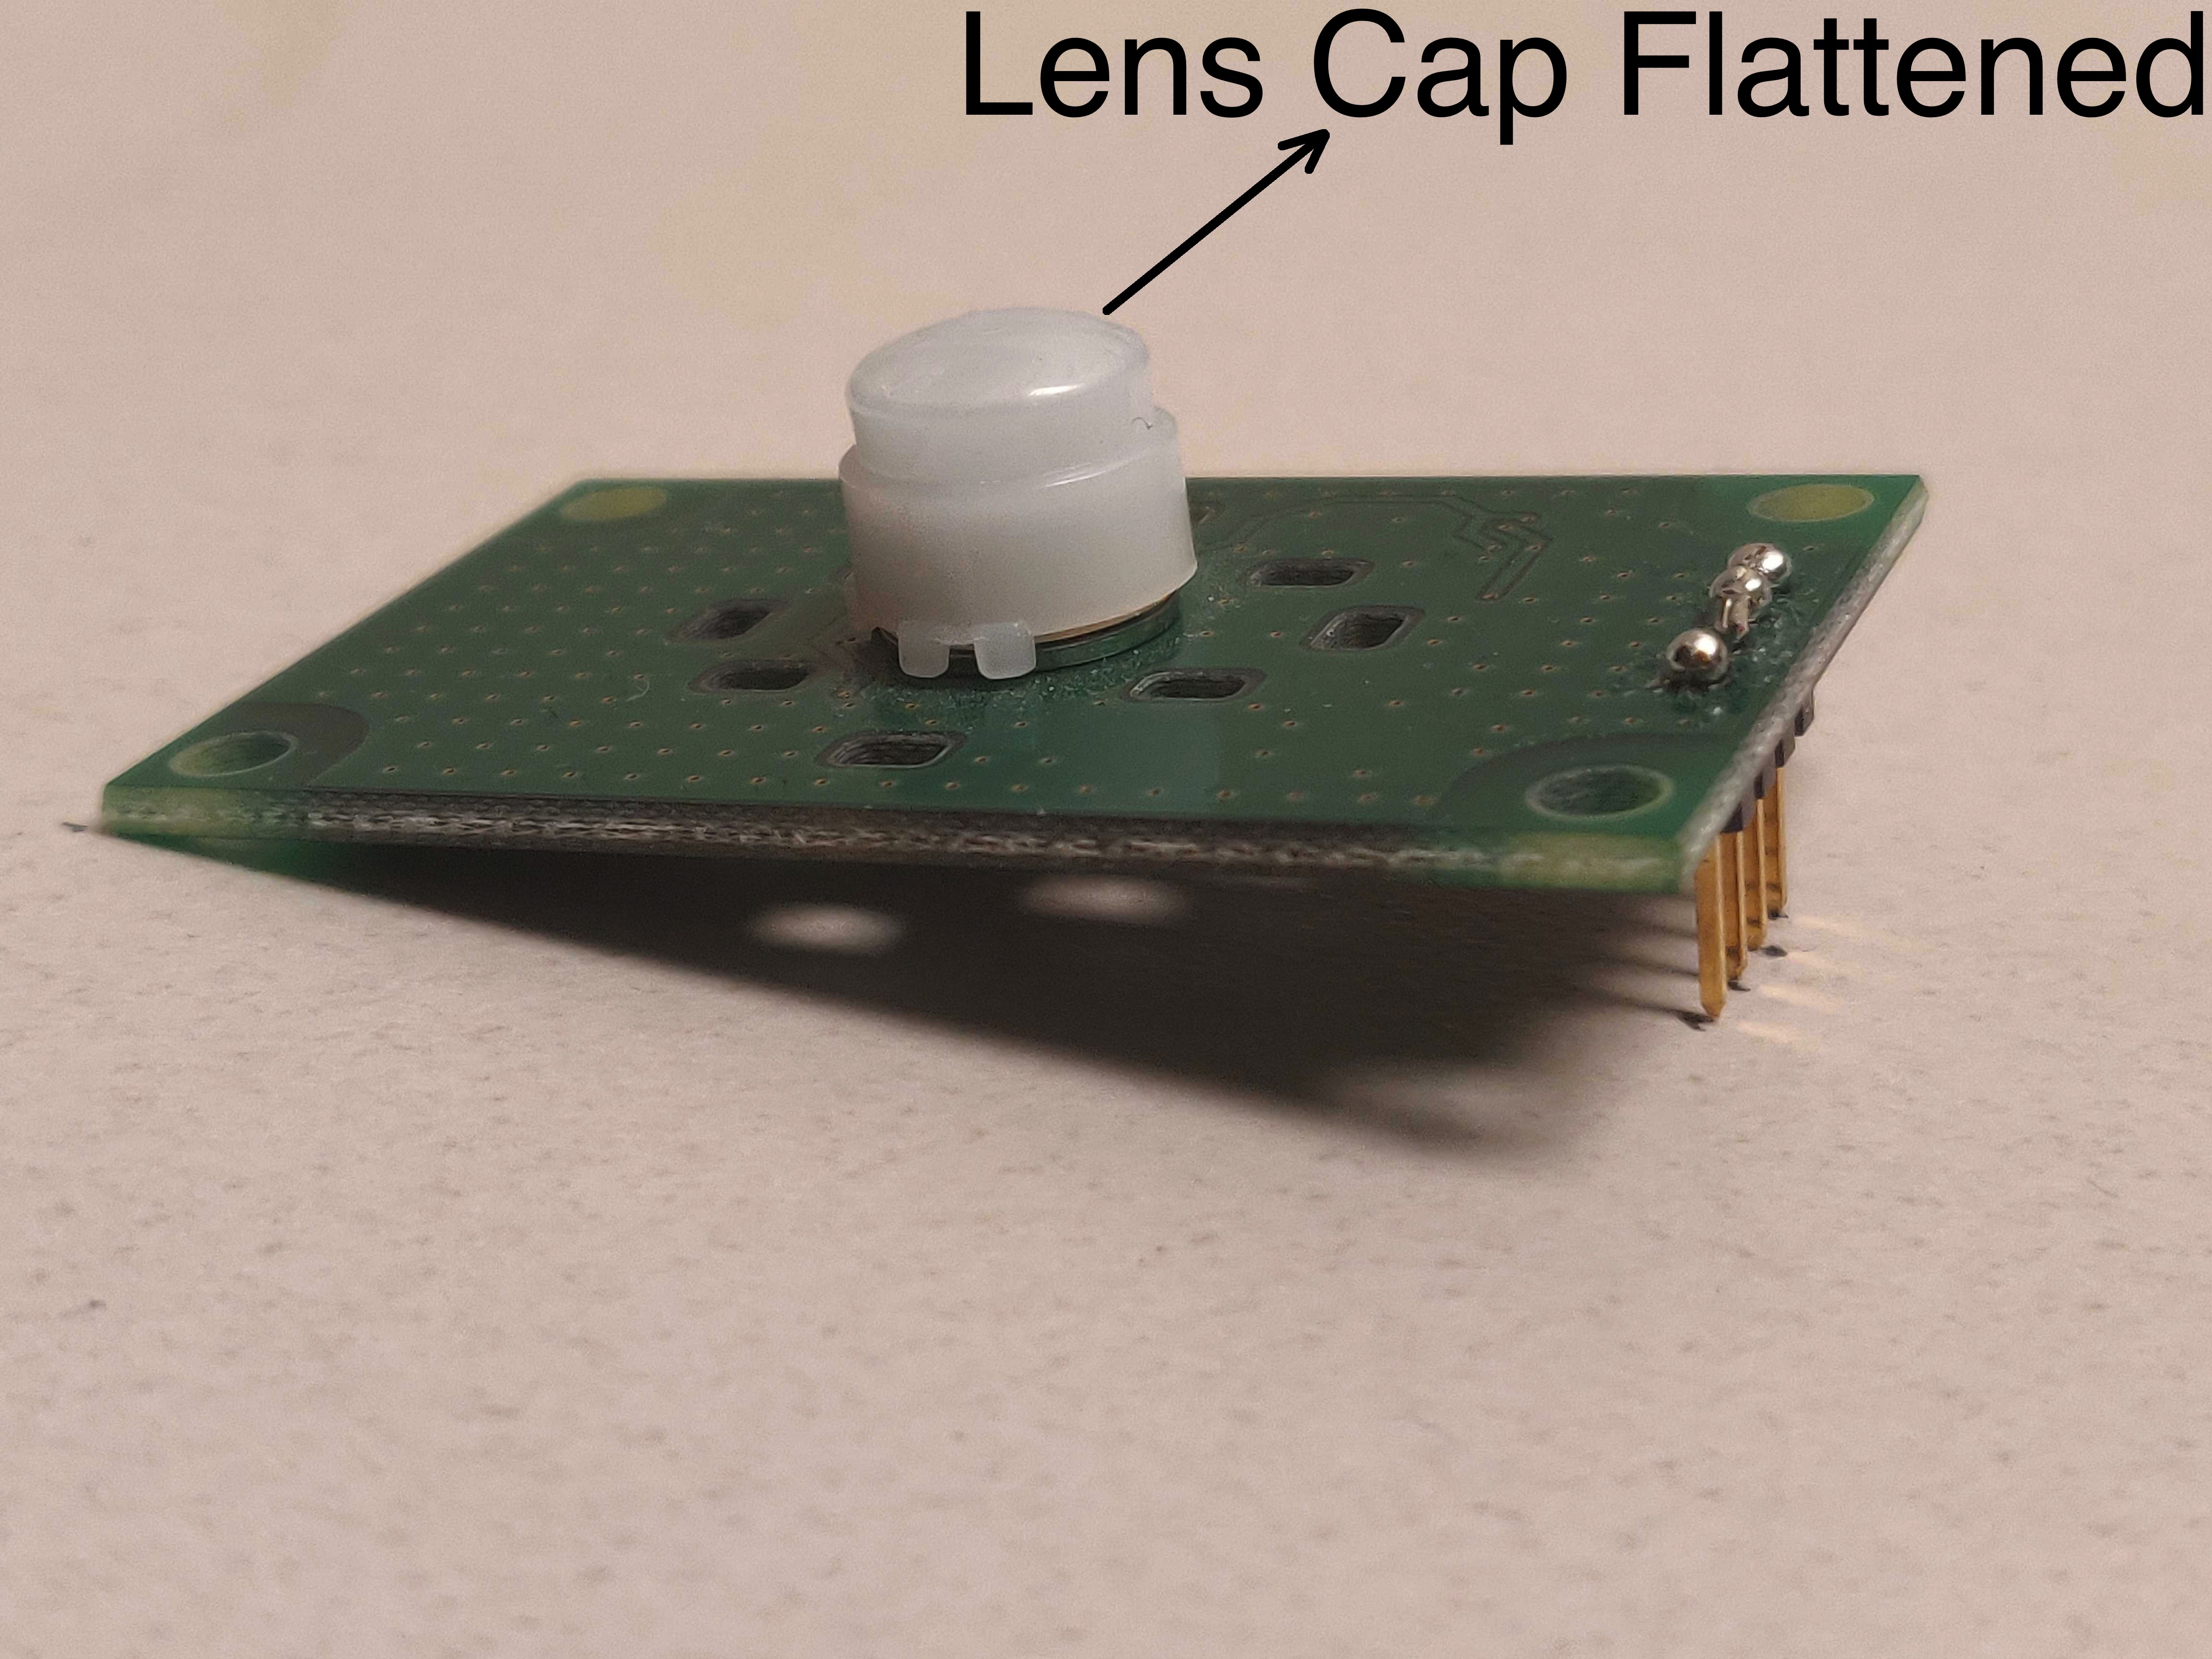
\includegraphics[width=\textwidth]{figures/platform/failure_photographs/ClassII-LensCapDeformed-annotated-jpg.jpg}
		\caption{Lens Cap Deformed}
		\label{fig:failure_photo3}
	\end{subfigure}
	\begin{subfigure}[t]{0.24\textwidth}
		\centering
		\includegraphics[width=\textwidth]{figures/platform/failure_photographs/ClassII-LensCapPunctured_new-2-annotated.png}
		\caption{Lens Cap Punctured}
		\label{fig:failure_photo4}
	\end{subfigure}
	\hspace{0.1ex}
	\begin{subfigure}[t]{0.24\textwidth}
		\centering
		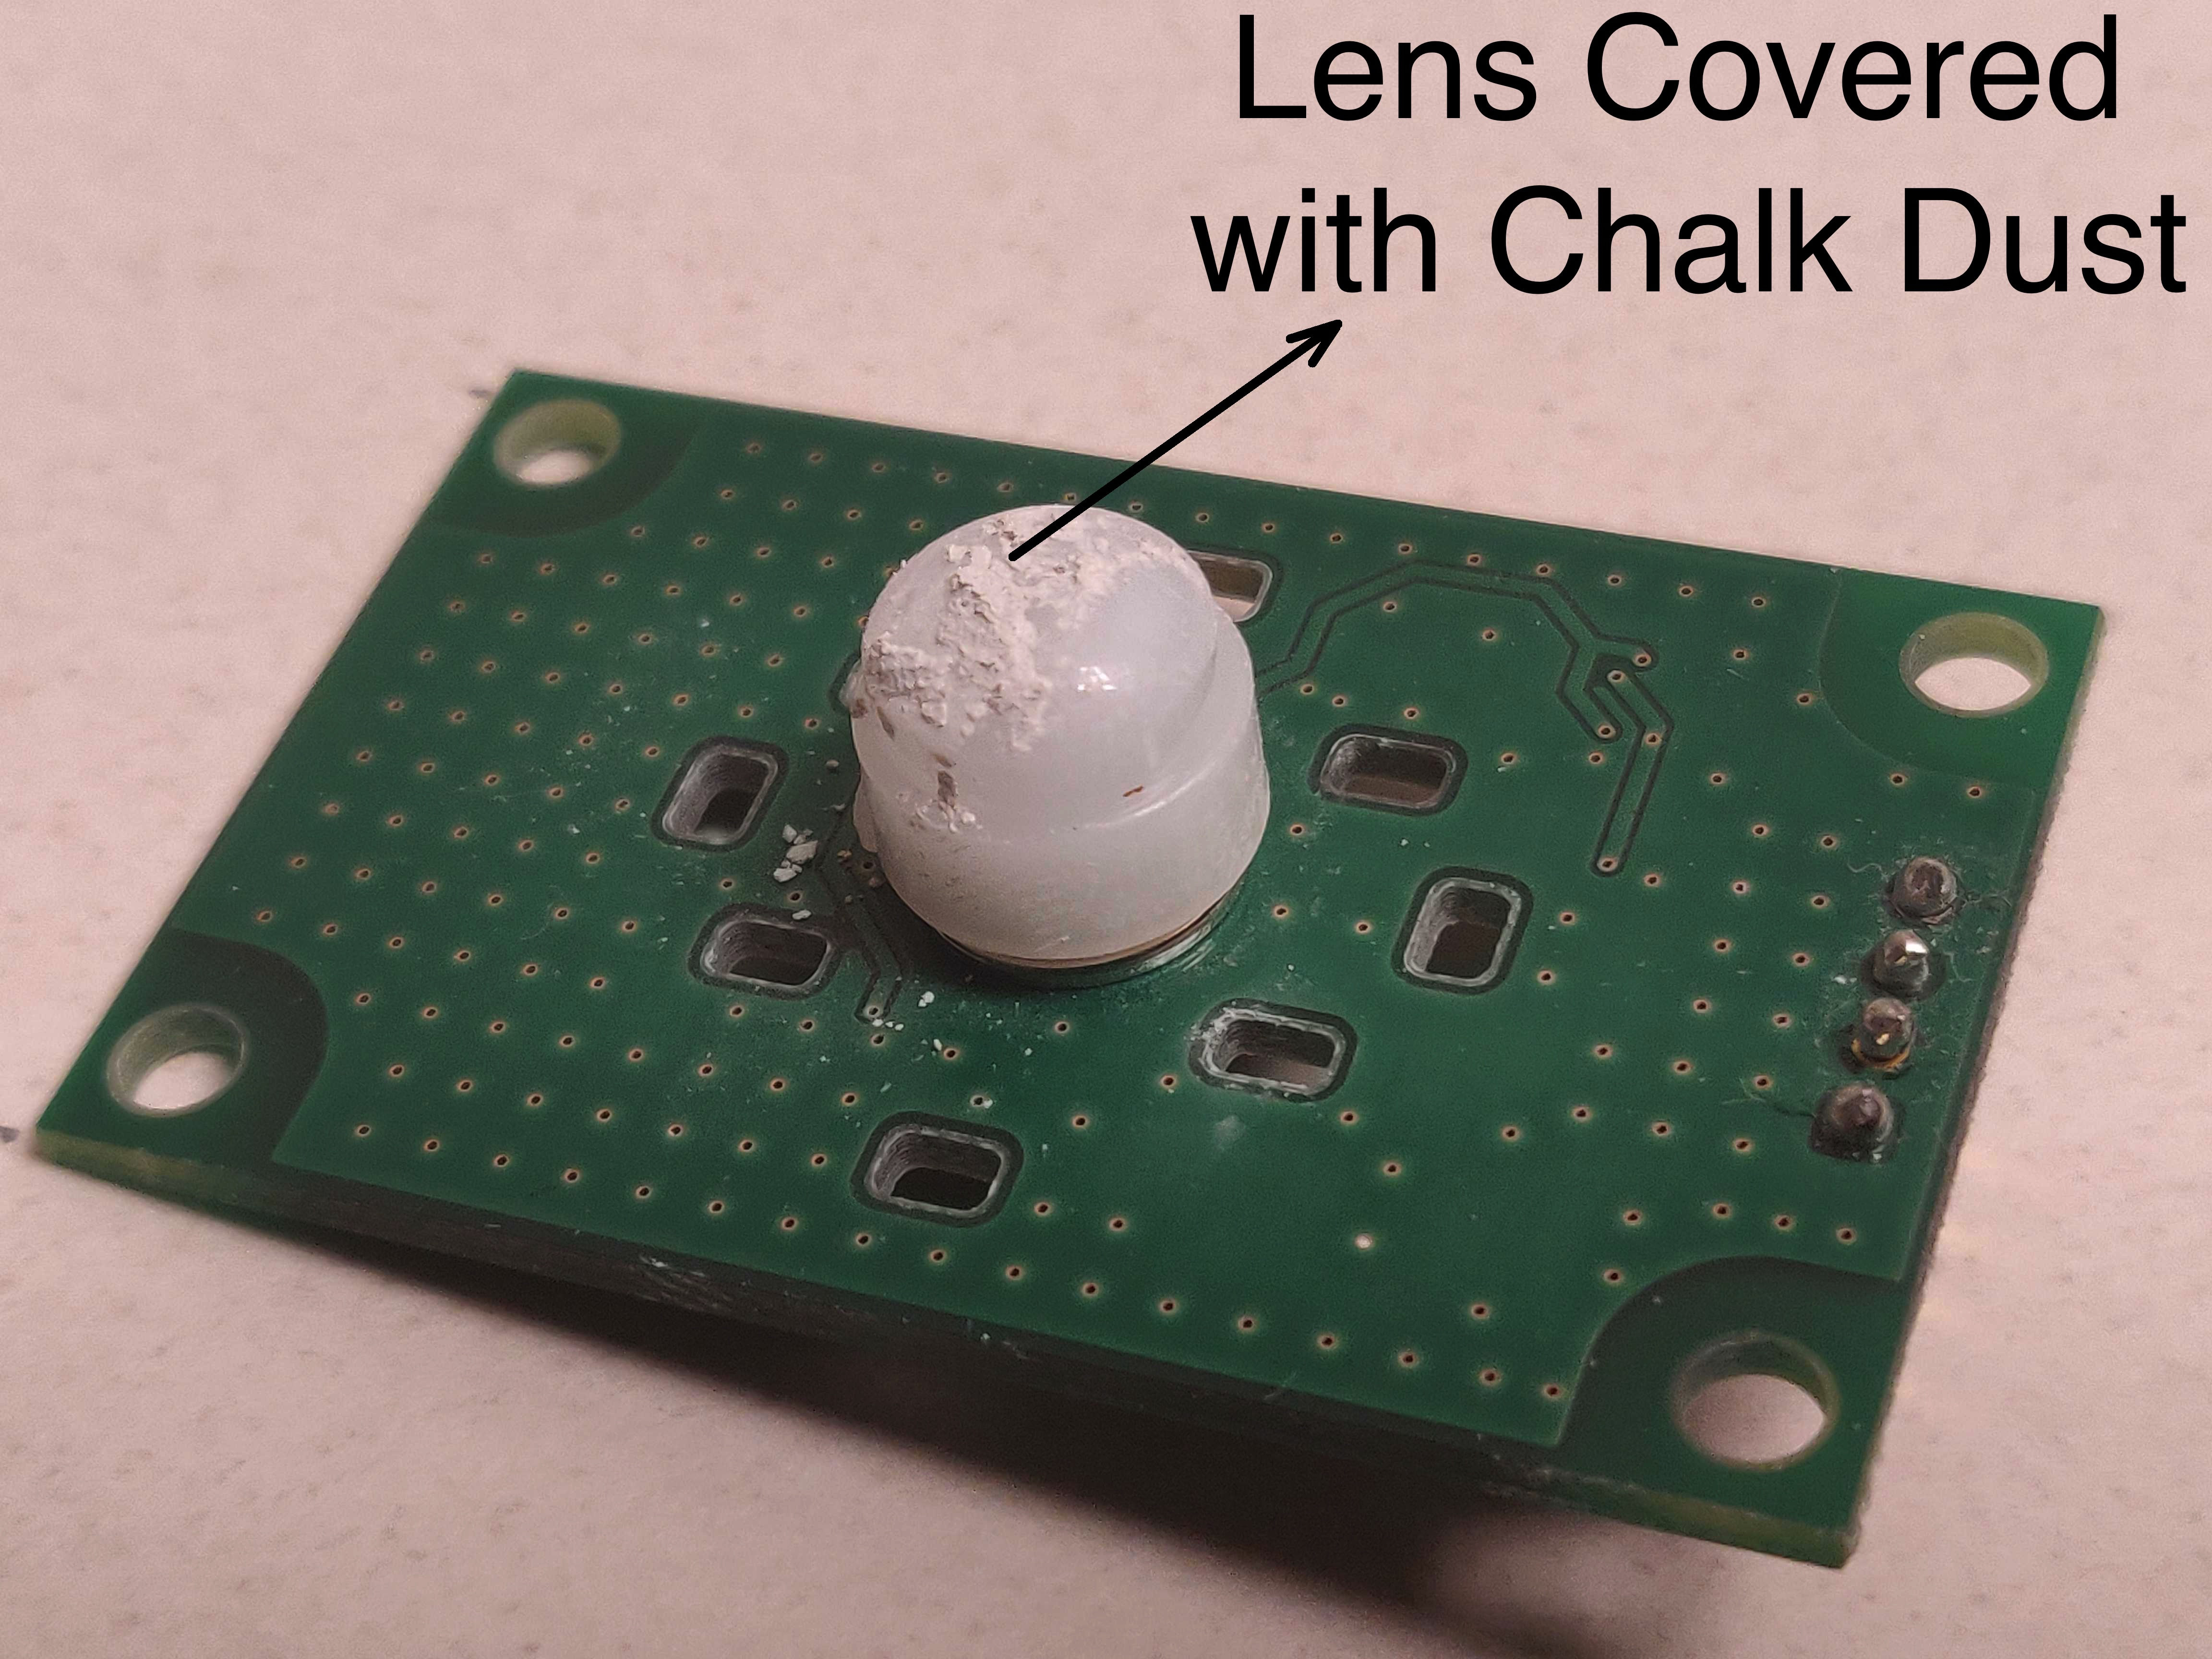
\includegraphics[width=\textwidth]{figures/platform/failure_photographs/ClassIII-LensCapCovered-annotated-jpg.jpg}
		\caption{\footnotesize Lens Cap Covered}
		\label{fig:failure_photo5}
	\end{subfigure}
	\hspace{0.1ex}%
	\begin{subfigure}[t]{0.24\textwidth}
		\centering
		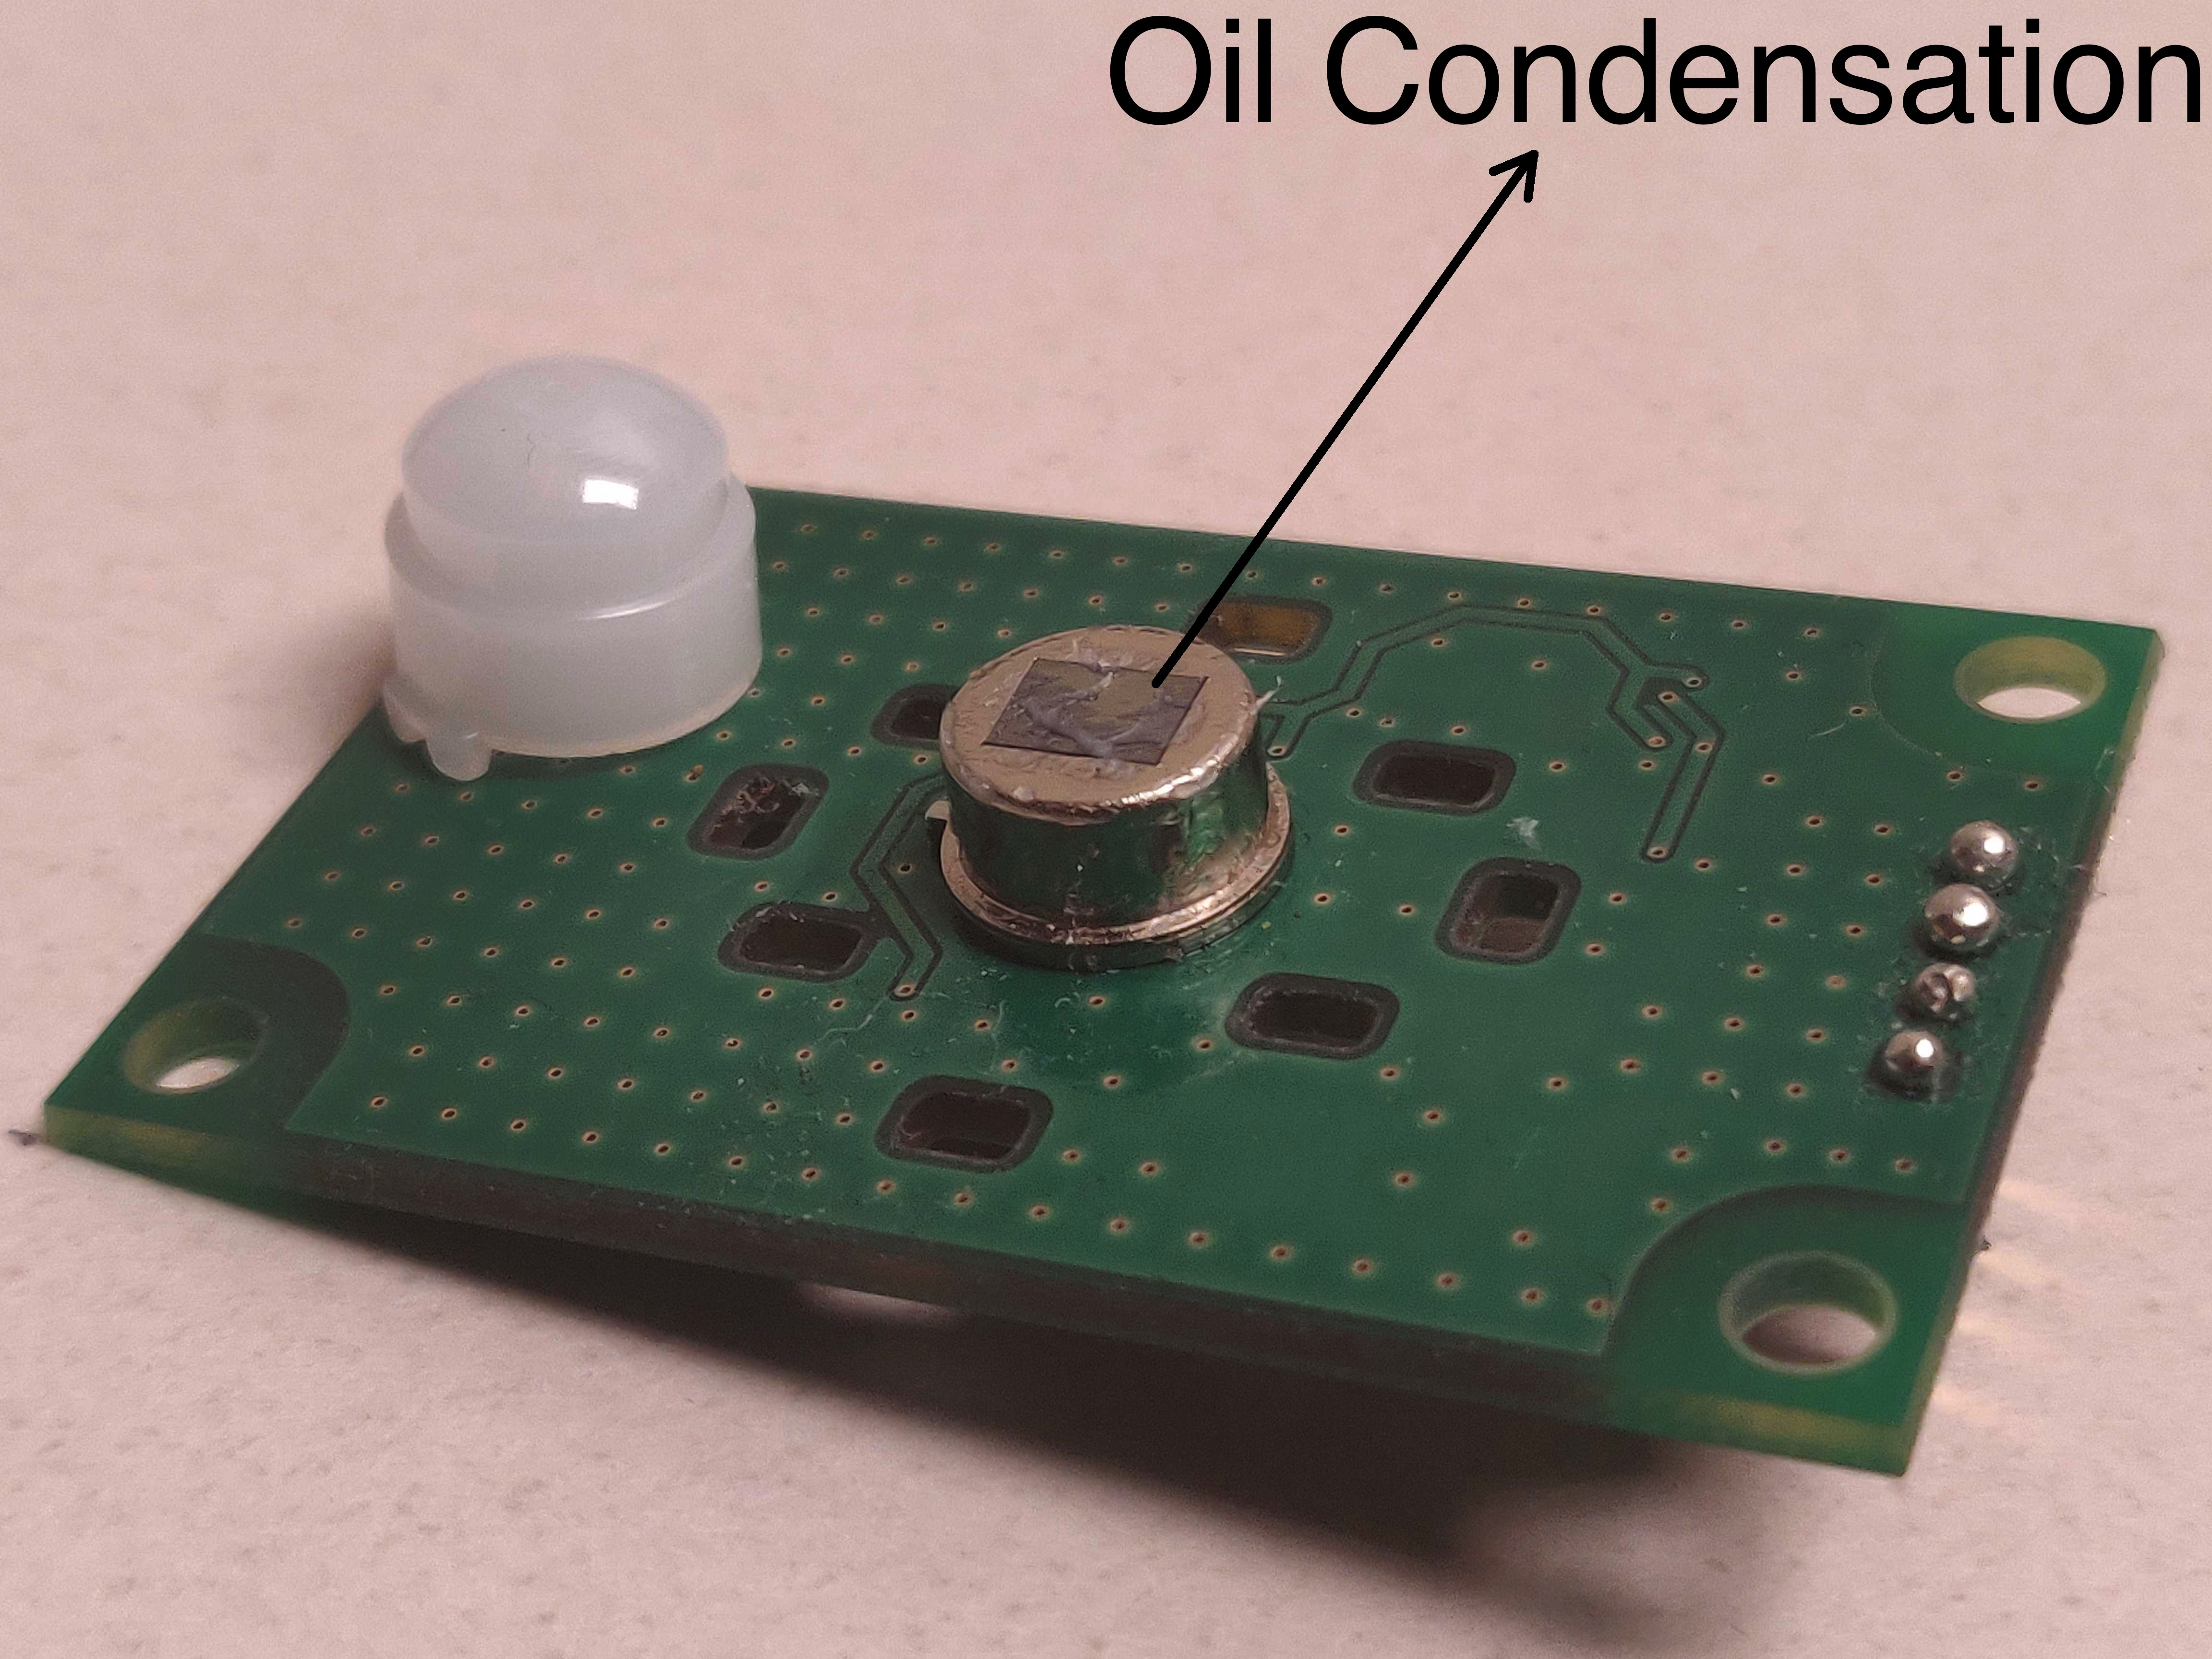
\includegraphics[width=\textwidth]{figures/platform/failure_photographs/ClassIV-OpticalFilterDamage-annotated-jpg.jpg}
		\caption{\footnotesize Optical Filter Damaged}
		\label{fig:failure_photo6}
	\end{subfigure}	
	\hspace{0.1ex}
	\begin{subfigure}[t]{0.24\textwidth}
		\centering
		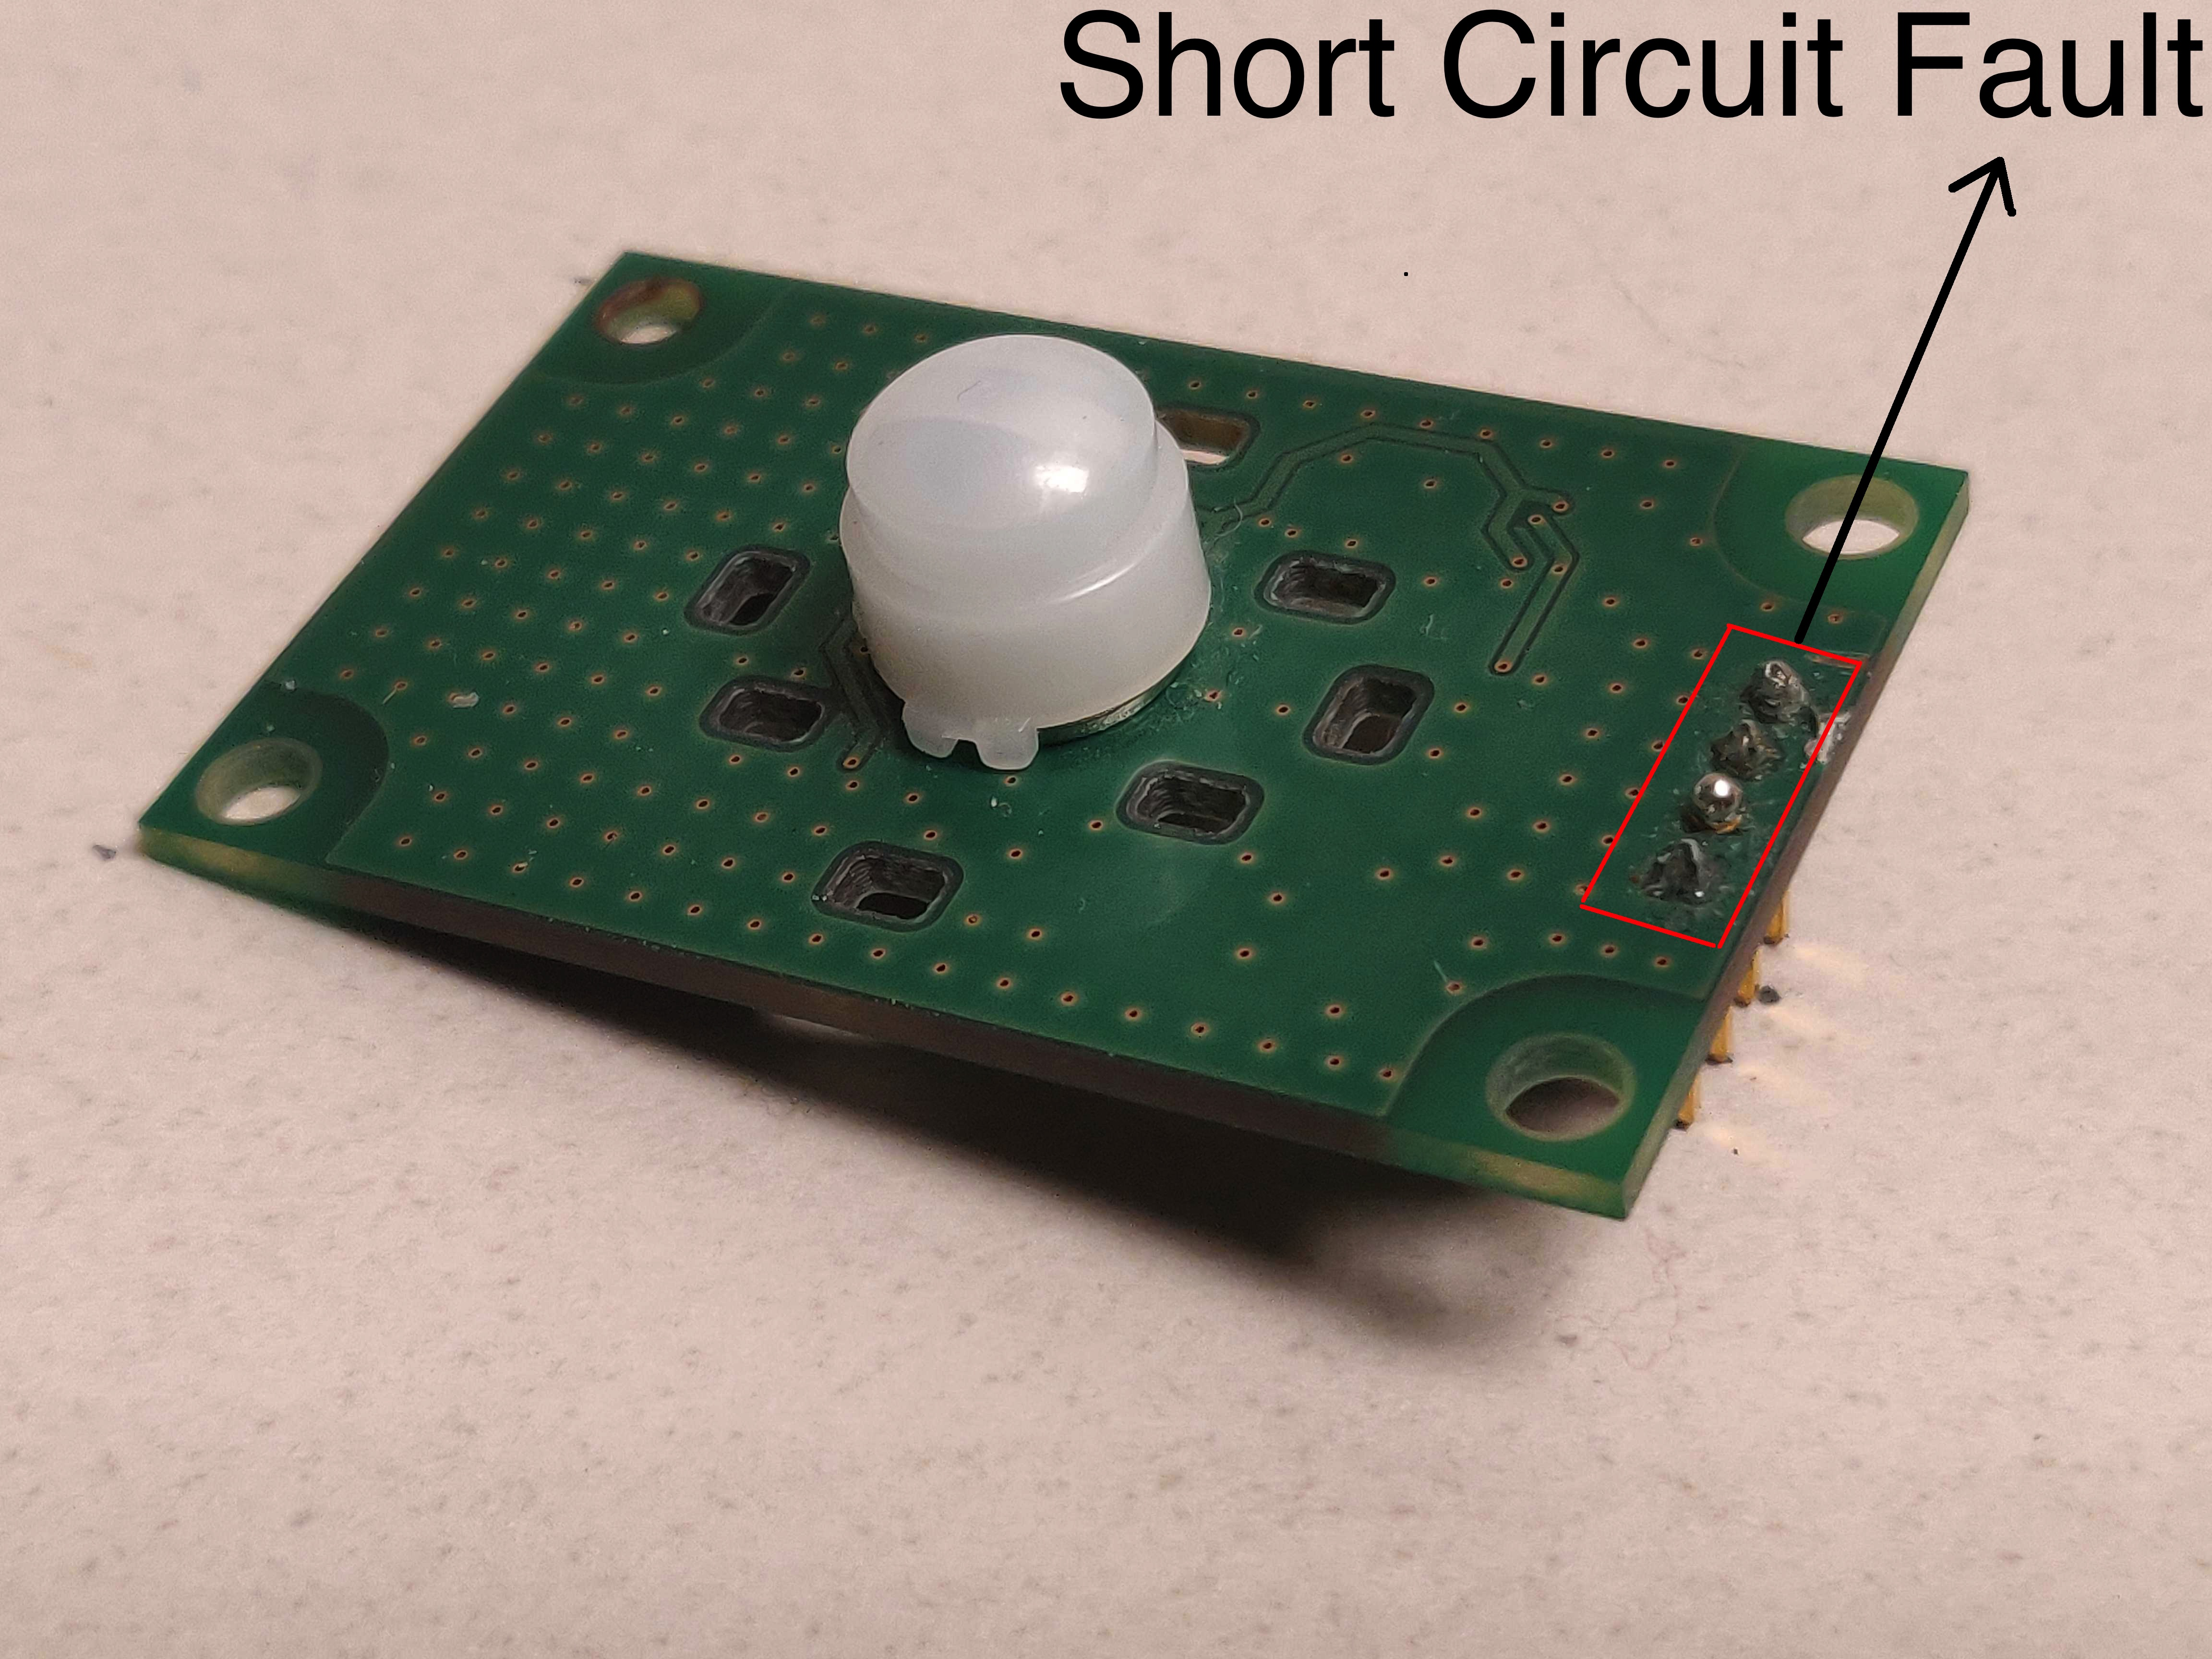
\includegraphics[width=\textwidth]{figures/platform/failure_photographs/ClassV-ElectronicsFault-annotated-jpg.jpg}
		\caption{Electronic Fault}
		\label{fig:failure_photo7}
	\end{subfigure}	
	\caption{\footnotesize{Some sensors} used in our study. Note that the failures are not always visually perceivable as the sensors are typically inaccessible.}
	\label{fig:pir_sensor_failure_photographs}
\end{figure}

\noindent \underline{Lens deformation (Class II):} As the lens is made of flexible, 0.4mm thick high density plastic~\cite{fresnel}, it is susceptible to deformation by physical damage. This can alter the curvature or puncture the lens. %
As in Class I, the consequence of failure is imperfect capture and focusing of the thermal radiation incident on the PIR sensor.

\noindent \underline{Lens hindrance (Class III):} Dust particles (\eg factory floors, building construction) or common objects such as paper and plastic tape can absorb the thermal radiation resulting in reduced to no radiation falling on the pyroelectric element. The deposition of particulate matter also causes dispersion.

In summary, Classes I--III failures affect the core functionality of the lens, and results in the imperfect capture and focus of thermal radiation.

\subsubsection{\textbf{Failures in the pyroelectric subsystem}: Optical Filter Damage (Class IV):} %
The optical filter and pyroelectric elements are prone to degradation with exposure to high temperature and humidity. As the optical filter is carefully calibrated to trigger in the region of human motion, it is susceptible to damage due to environmental factors such as heat sources (\eg room heaters, air-conditioners) and humidity (\eg oil condensation) as it affects the perceived temperature of the object. We name these as Class IV failures.

\subsubsection{\textbf{Failures in the Electronics}} On-board electronics consisting of filter, amplifier and comparator circuitry are prone to failures such as shorted or floating pins that we refer to as Class V failures. We only consider simple, electronic failures -- such as open, short circuits and floating inputs. Vendor-based IC testing procedures and board design process advancements have made electronic failures such as regulator, bus failures and PCB malfunctions infrequent in practice.
%
%

\noindent \textbf{Summary:} Failures in PIR sensors can occur in either the lens subsystem, the pyroelectric subsystem or the on-board electronics, each of which manifest differently in the underlying physics.

\begin{wraptable}{lr}{0.6\textwidth}%
	\centering
	\footnotesize
	\caption{{\bfseries Taxonomy of Failures} in a PIR Sensor}
	\begin{tabular}{p{2.25cm} p{6cm}}
		\hline %
		\textsc{\bfseries Failure} & \textsc{\bfseries Definition \& Impact}\\
		\hline\hline
		\rowcolor{gray!20} \multicolumn{2}{l}{\bfseries Lens Subsystem}\\
		Lens dislodged \newline (Class I) & Lens cap suffers partial or complete dislocation \eg physical impact with a foreign object, degradation of bonding,~\etc \\
		Lens deformed \newline (Class II) & Lens cap suffers physical damage in-place \eg deformation, puncture,~\etc \\
		Lens covered \newline (Class III) & Lens cap gets physically obstructed by foreign particles \eg dust, paper or tape \\
		\hline
		\rowcolor{gray!20} \multicolumn{2}{l}{\bfseries Pyroelectric Subsystem} \\
		Optical filter \newline damage (Class IV) & Damaged by environmental factors~\eg oil condensation\\
		\hline
		\rowcolor{gray!20} \multicolumn{2}{l}{\bfseries Electronic Subsystem} \\
		Electronic faults \newline (Class V) & Hardware failures~\eg short circuits, floating outputs~\etc \\
		\hline
	\end{tabular}
	\label{tab:pir_faults}
\end{wraptable}

\subsection{Analyzing Severity of Failures -- A Quantitative Analysis}
\label{subsec:quantify}
A failure is said to impact the sensor performance if the failure results in either false detections ({\bfseries FD}) \ie false positives or missed obstacles ({\bfseries MO}) \ie false negatives in the sensor output (\cout), compared to a working sensor. As seen in {\bfseries Fig.~\ref{fig:pir_sensor_different_lens}}, \cout is HIGH (1) when no is obstacle detected and \cout goes HIGH (1) $\rightarrow$ LOW (0) when an obstacle is detected.

\noindent \underline{Controlled Failure Study:} To understand the impact on sensor performance, in our lab, we take 2 PIR sensors, one which is without the fault (\working) and one with the fault (\tampered). The 2 sensors are placed in as close a proximity to one another as possible such that -- \ca distance between the sensors are closer than the size of obstacle, \cb the obstacle is moved in a plane such that it comes into the detection region of both the PIR sensors simultaneously. This implies that when the obstacle (we used our palm in this case) is moved across the detection region of both PIR sensors, it grazed both at the same time, triggering the same responses from both the sensors.

We then calculate the absolute difference ($\delta_N$) between the \cout values of the tampered sensor~\viz  \couttampered and the reference working sensor~\viz \coutworking by summing over all observations (Refer Eqn.~\ref{eqn:1}). Intuitively, a relatively low $\delta_N$ would imply that the tampered sensor is still in acceptable condition \ie the failure is not having much impact on the operation of the sensor. On the other hand, a high value of difference implies that the failure is much serious. To ease computation, we can also compute $\delta_N$ by dividing the time series into equal size chunks called \textit{windows} (W) and computing the difference between average \cout values of \tampered and \working in that window.

\begin{table}%
	\small
	\centering
	\caption{\textbf{Misclassifications} analysis for different failures. The numbers indicate the deviation (as defined in Eqn.~\ref{eqn:1} between $C_{out}$ values) of a faulty sensor from that of a working sensor. Higher number indicates increased degree of failure.}
	\begin{tabular}{lllll}
		\hline
		\bfseries \textsc{Failure} & \bfseries \textsc{Lens Dislodged} & \bfseries \textsc{Lens Covered} & \bfseries \textsc{Heat Damage} & \bfseries \textsc{Humidity Damage}\\
		\hline \hline
		\rowcolor{gray!20} $\delta_N$$^1$ & 35 & 48 & 29 & 48 \\
		$\delta_N$$^2$ & 69 & 94  & 53 & 87 \\
		\hline 
	\end{tabular}
	\label{tbl:fault_degree}
	\quad \raggedright
	$^1$ 6 hour run, $^2$ 12 hour run
\end{table} 

\textbf{Table~\ref{tbl:fault_degree}} summarizes $\delta_N$ for a few types of failures as observed over 6-hour and 12-hour runs deployed in the elevator of our building. The numbers in the column represent deviation or misclassifications ($\delta_N$)~\ie the number of false detections (both false positives and false negatives) by the faulty sensor calculated using {\bfseries Eqn.~\ref{eqn:1}}.
We used a window size, $W$ = 1024 samples, which comes to a window of time duration slightly over 51 seconds at a sampling rate of 20 Hz.
In our case, the lens covered failure (8 failures per hour) is more pernicious than lens having fallen off (6 failures per hour).

\begin{equation}
	{\tikzmarknode{d}{\highlight{blue}{$\delta_N$}}} = \underset{windows}{\sum} 
	\left| {\tikzmarknode{t}{\highlight{red}{$C_{\text{out,tampered}}$}}} - {\tikzmarknode{w}{\highlight{green}{$C_{\text{out, working}}$}}}\right|,
	\label{eqn:1}
	\begin{tikzpicture}[overlay,remember picture,>=stealth,nodes={align=left,inner ysep=1pt},<-]
		\path (d.south) ++ (0,-0.6em) node[anchor=north east,color=blue!67] (scalep){\textbf{misclassifications}};
		\draw [color=blue!57](d.south) |- ([xshift=0.3ex,color=red]scalep.south west);
	\end{tikzpicture}
	\begin{tikzpicture}[overlay,remember picture,>=stealth,nodes={align=left,inner ysep=1pt},<-]
		\path (t.north) ++ (0,0.6em) node[anchor=south east,color=red!67] (scalep){\textbf{tampered}};
		\draw [color=red!57](t.north) |- ([xshift=-12ex,color=red]scalep.south east);
	\end{tikzpicture}
	\begin{tikzpicture}[overlay,remember picture,>=stealth,nodes={align=left,inner ysep=1pt},<-]
		\path (w.north) ++ (0,0.6em) node[anchor=south west,color=teal] (scalep){\textbf{working}};
		\draw [color=teal!57](w.north) |- ([xshift=-0.3ex,color=green]scalep.south east);
	\end{tikzpicture}
\end{equation}\\



\noindent \textbf{Summary:} Quantifying the impact of a failure gives hints on how pernicious specific failures are \textit{once they have been detected}.%




\begin{figure}[b]
	\centering
	\begin{subfigure}[b]{0.3\textwidth}
		\centering
		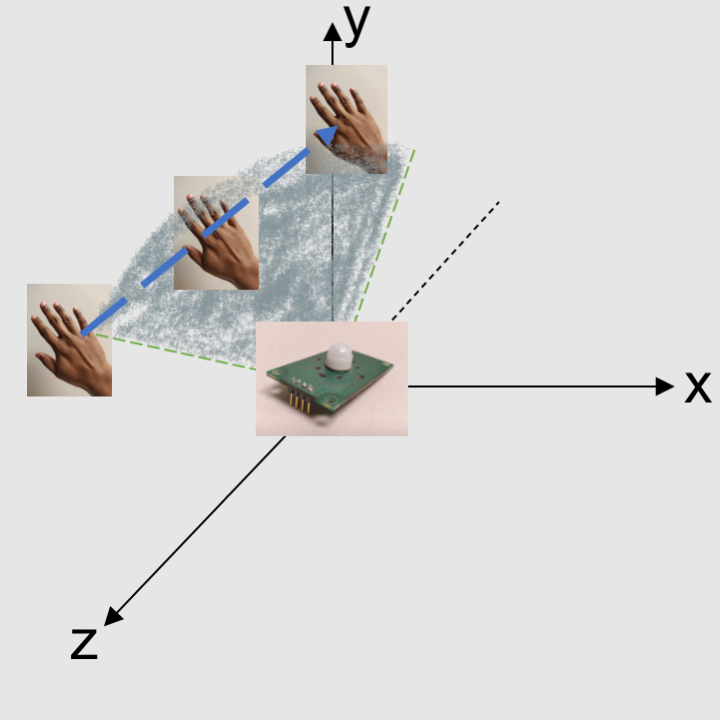
\includegraphics[scale=0.6, height=1.3in]{figures/platform/controlled_setup-2.png}
		\caption{Controlled Setup}
		\label{fig:pir_sensor_controlled}
	\end{subfigure}%
	\begin{subfigure}[t]{0.3\textwidth}
		\centering
		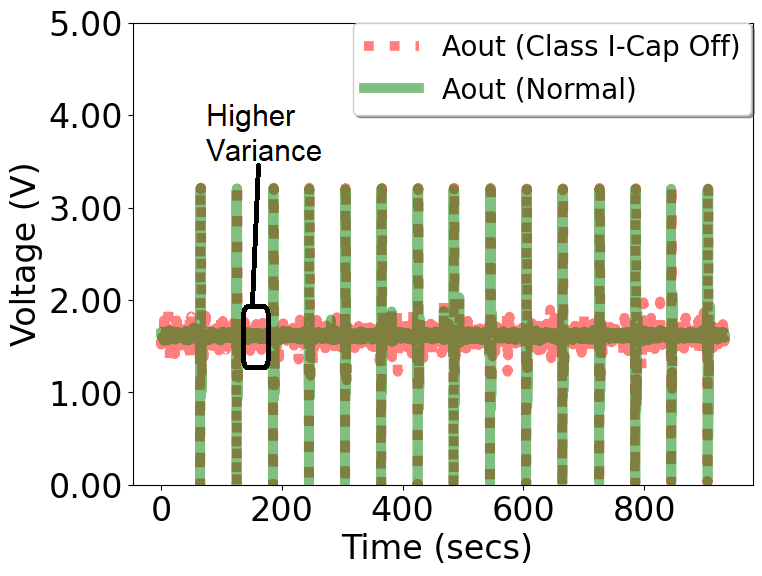
\includegraphics[width=\textwidth]{figures/2-PIR-Fault/normal-classI/classI_compared-again.png}
		\caption{Class I Fault}
		\label{fig:pir_sensor_controlled_a}
	\end{subfigure}%
	\begin{subfigure}[t]{0.3\textwidth}
		\centering
		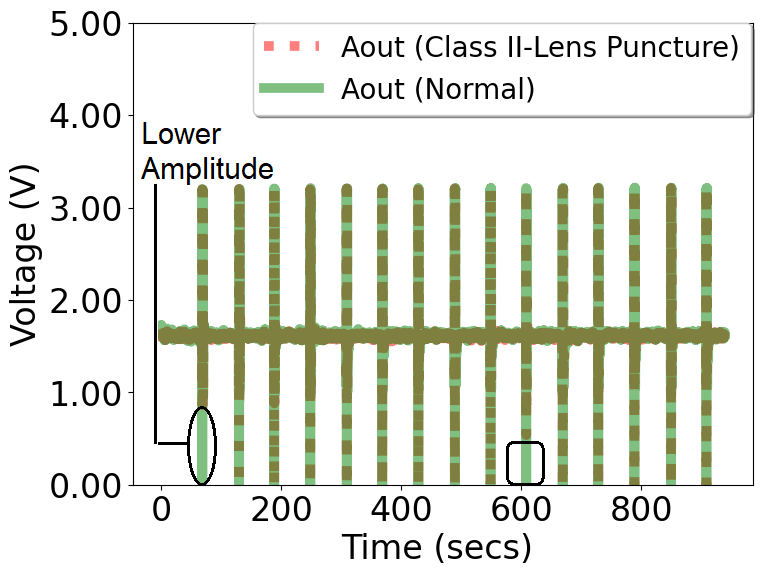
\includegraphics[width=\textwidth]{figures/2-PIR-Fault/normal-classII/classII_compared.png}
		\caption{Class II Fault}
		\label{fig:pir_sensor_controlled_b}
	\end{subfigure}\\%
	\begin{subfigure}[t]{0.3\textwidth}
		\centering
		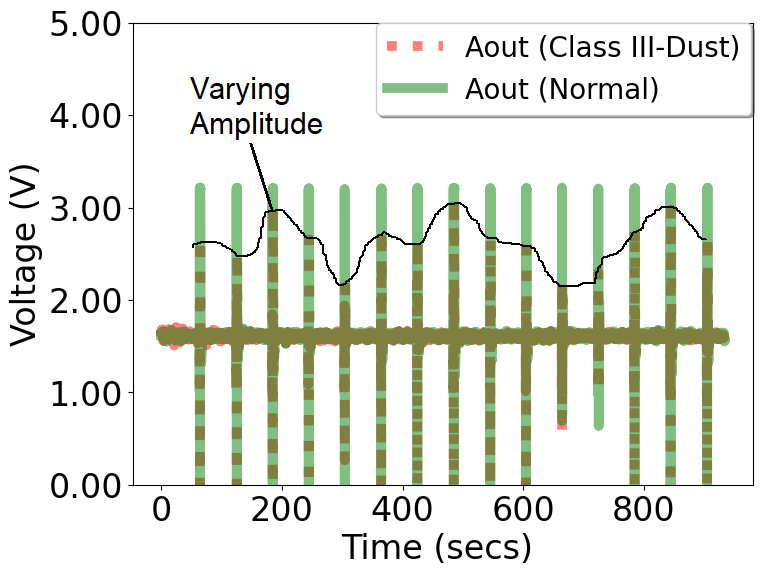
\includegraphics[width=\textwidth]{figures/2-PIR-Fault/normal-classIII/classIII_compared.png}
		\caption{Class III Fault}
		\label{fig:pir_sensor_controlled_c}
	\end{subfigure}
	\begin{subfigure}[t]{0.3\textwidth}
		\centering
		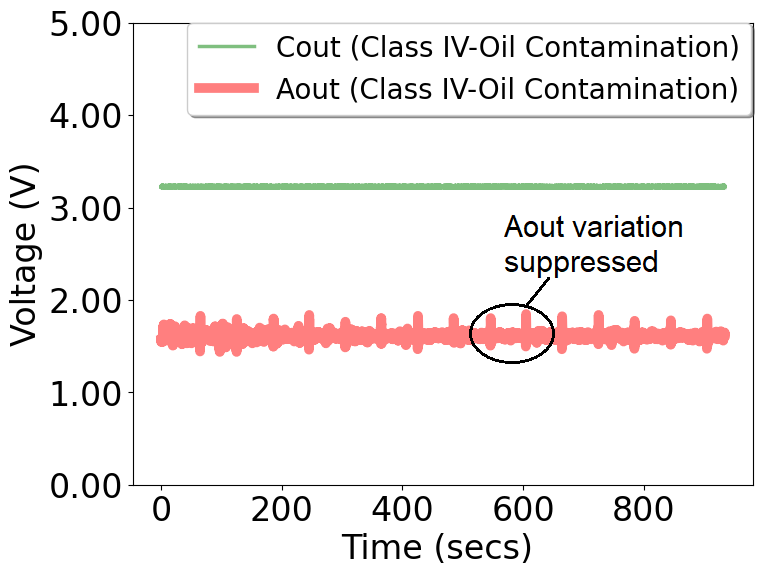
\includegraphics[width=\textwidth]{figures/2-PIR-Fault/normal-classIV/classIV_summary.png}
		\caption{Class IV Fault}
		\label{fig:pir_sensor_controlled_d}
	\end{subfigure}%
	\begin{subfigure}[t]{0.3\textwidth}
		\centering
		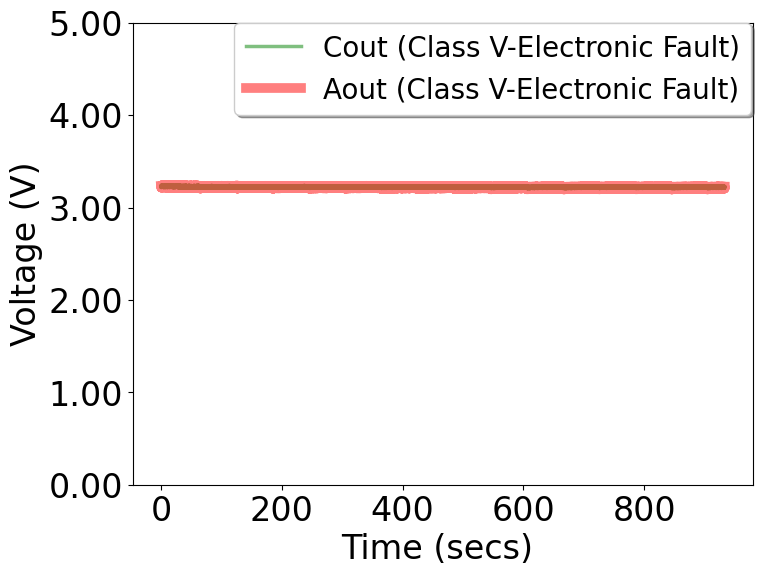
\includegraphics[width=\textwidth]{figures/2-PIR-Fault/normal-classV/classV_summary.png}
		\caption{Class V Fault}
		\label{fig:pir_sensor_controlled_e}
	\end{subfigure}
	\caption{(\ref{fig:pir_sensor_controlled_a} - \ref{fig:pir_sensor_controlled_e}) \footnotesize{\aout waveforms for sensor faults of Classes I--V}. Note that in Class I -- III faults, despite the obstacle still being detected, \aout provides indication of underlying abnormalities in the sensor.
	}
	\label{fig:pir_sensor_controlled_classI-V}
\end{figure}





